\documentclass[11pt]{article}

\textwidth 17cm
\textheight 23cm
\oddsidemargin 0.25cm
\addtolength{\voffset}{-2.4cm}
\addtolength{\hoffset}{-0.5cm}

\setlength{\parindent}{12pt}
\setlength{\parskip}{3pt}
\usepackage{float, comment}

%\usepackage{refcheck}

%\usepackage[caption = false]{subfig}

\usepackage{amssymb,amsmath,epsfig}

%\usepackage[colorlinks=true,breaklinks=true,linkcolor=black,citecolor=black]{hyperref}

\usepackage{graphics,psfrag,graphicx,color,float,subcaption} %amsthm

\numberwithin{equation}{section}
%\numberwithin{figure}{section}

\usepackage[table]{xcolor}

\usepackage{textpos}

% OUR DEFINITIONS %%%%%%%%%%%%%%%%%%%%%%%%%%%%%%%%%%%
\usepackage{sebastyle}
\DeclareMathAlphabet\mathbfcal{OMS}{cmsy}{b}{n}

\newcommand{\rred}[1]{\textcolor{red}{#1}}
\newcommand{\ccite}{\rred{****CITE HERE****}}
% END OF OUR DEFINITIONS %%%%%%%%%%%%%%%%%%%%%%%%%%%%%

%\allowdisplaybreaks

%***********************************************************************************

\title{New techniques and technologies in data driven approaches to sustainability
\thanks{This research was 
partially supported by  Pacific Institute for the Mathematical Sciences, Mitacs, QuanSight, West Grid and Cybera.}}

\author{
{\sc Symon Islam}\thanks{Department of Mathematics, Simon Fraser University, Canada.
email: {\tt symonyeal@gmail.com}.}
\and
{\sc Sebasti\'an Moraga}\thanks{ Department of Mathematics, Simon Fraser University, Canada.
email: {\tt smoragas@sfu.ca}.}
\and
{\sc Edgar Pacheco}\thanks{Department of Mathematics and Statistics, University of Calgary, Canada.
email: {\tt edgar.pachecocastan@ucalgary.ca}.}
\and
{\sc Thomas Pender}\thanks{Department of Mathematics and Computer Science, University of Lethbridge, Canada.
email: {\tt thomas.pender@uleth.ca}.}
\and
{\sc Igor Pinheiro}\thanks{Department of Mathematics, University of British Columbia, Canada.
email: {\tt igor.ivpp@math.ubc.ca}.}
}

\date{}

\begin{document}

\maketitle
\begin{textblock*}{2cm}(0cm,-5.5cm)
  
\includegraphics[scale=0.1]{m2pilogo}%\rule{2cm}{1cm}
\end{textblock*}

\begin{abstract}
\noindent In this paper, we study several aspects of sustainability in agriculture. The need to provide information and projections to farmers and producers is addressed. Then we study several indicators of the environmental impacts on agricultural production.
\end{abstract}

\begin{comment}
\noindent
{\bf Key words}: Machine learning, agriculture, climate change, optimization, water
\end{comment}

\smallskip\noindent

                                                  
%%%%%%%%%%%%%%%%%%%%%%%%%%%%%%%%%%%%%%%%%%%%%%%%%%%%%%%%%%%%%%%%%%

\section{Introduction}\label{introduction}

Sustainability is the greatest challenge facing the human race, and in the face of global warming coupled with population increase, the strain on vital sectors, like agriculture, is mounting at an accelerated pace. This project is focused on the use of open data to improve understanding, and, ideally, predictability, for the environmental impact from agriculture. 

Agriculture is one of the most significant areas of economic activity for countries around the world, and it has a significant environmental impact; it is estimated that agriculture accounts for at least $10\%$ of green house gas emissions in many countries. In nearly every country, there is an impact from agricultural practices through changing land use, water consumption, use of fertilizer, GHGs and other emissions. From a local perspective agriculture creates different dynamics for indigenous plant and animal life in addition to creating different micro-climates. On a more broad scale, agriculture can put pressure on entire river systems and lead to changing weather patterns as atmospheric humidity and solar radiation emissions change.

The ideal outcome of this project is the design of a model and a system of action for environmental impacts that leverages open data and provides a complement to the current TheoryMesh system which is capturing operational impacts from farm activities. Invariably, the project and its outcome will be data driven.

There are many data sources available to investigate environmental changes and impacts due to agriculture. Furthermore, there is a proliferation of data sets that convey information about practices, agricultural production, and green house gas emissions. Combining data across data sources and interpreting the data in new ways could provide better insights on sustainability. Using machine learning techniques to creating models to describe these impacts could improve planning and shift practices to reflect longer term environmental impact. For example, technologies like Blockchain may provide a foundation to create an immutable data ledger for environmental impact while also leveraging smart contracts to take action on data when conditions are met.

For a broader view, the reader is encouraged to read The United Nations Sustainable Development Goals that describe a multi-faceted view of sustainability covering environment, economic and societal factors \cite{UN-edgar}.

Finally, we note that tables and figures are reserved for an Appendix at the end of this document.

%%%%%%%%%%%%%%%%%%%%%%%%%%%%%%%%%%%%%%%%%%%%%%%%%%%%%%%%%%%%%%%%%%

\section{Models and results}\label{Corr_modl}

In this section we discuss briefly the models used on the data collected  in this research. The models we implemented are simple linear regresion models of the type 
\begin{equation}
Y_i = \beta_0 + \sum_{j=1}^k \beta_j X_{i,j},    
\end{equation}
 for the observations $i\in \{1, 2, \dots, N\}$, where $N$ are total number of observations, and where thre are dependent variables $k$.
 
 Furthermore, in this study we use the dependence between two specific quantities using  a correlation coefficient matrix, with  the Pearson's correlation coefficients. This method is widely used to see linear correlation between variables that also uses a least squares fitting to the data obtained.

 %%%%%%%%%%%%%%%%%%%%%%%%%%%%%%%%%%%%%%%%%%%%%%%%%%%%%%%%%%%%%%%%%%
 
\section{Problems}\label{problems}

The issues elluded to above are broad, and they are difficult to quantify and to analyze; indeed, agricultural sustainability is a function of a large number of variables. In an effort to make the problem more tractable, we focused on two smaller problems.

The first problem arose in the following way. There is a lot of work being done on the broader, macro scale. However, it is interesting that not much work has been done on the local, micro level. For instance, a common complaint among contemporary farmers is that information cannot be compiled and disseminated in the same ways anymore. It used to be the case that a producer might say ``Plant this crop on this day because that is what has always worked.'' This is no longer tenable with the changing climate and increased weather volatility.

All this is to say that the productivity of agricultural fields, what producers depend on, is being negatively affected, and new approaches to collecting, interpreting, and disseminating relavent information need to be produced.

As a second problem, we see that environment problems  have been a real matter in the last century. Factors that could be correlated can explain why certain aspects of area of production can affect others. The main issue here is,  to try to identify  factors in  Canada where an increasing (or decreasing) of them can  impact the environment and the surroundings. 

%%%%%%%%%%%%%%%%%%%%%%%%%%%%%%%%%%%%%%%%%%%%%%%%%%%%%%%%%%%%%%%%%%

\subsection{Productivity of Canadian Farms}\label{productivity}

There are many areas in the world that are experiencing the catastrophic effects of climate change. In the Middle East, many of the farmers who have had to rely on local tributaries to sustain their crops are having to to consider different ways of life as water levels of these rivers and lakes decrease and, ultimately, disappear. As these climate events unfold, the UN \cite{UN} warns of a proliferation of conflict over the increase in water scarcity.

For more northern regions, like Canada, the situation may develop differently. As the climate warms, areas to the north will continue to become more viable for a greater variety of agricultural practices and commodities. For instance, consider the length of the frost free days in the province of Alberta \cite{climate-data}.

In each climate model, where we note that rcp26, rcp45, and rcp85 are, respectively, the low, mid, and high emisions models, and as indicated by Figure \ref{ABfrostdays}, the number of consecutive frost free days will invariably increase. With the increased length of the growing season, there will be more opportunities to grow a greater variety of crops in regions that have been hitherto difficult to cultivate.

There are other climate variables to consider as well. Observe the cummulative monthly mean temperature in Alberta over the consecutive frost free days shown in Figure \ref{ABmeantemp} \cite{climate-data}.

These climate projections per locale can be used by producers in order to project at what points they may profitably consider changes in the location of their business and the type of crops they choose to grow in these locations.

To further evince the increasing productivity of Canadian crop yields, and to provide specific crop data per locale for producers, we can consider data like that shown in Figure \ref{ABbarleyyields}, which shows the change in barley yields in Alberta \cite{stat-can}. 

Assuming the yield to a be a function time and a number climate variables, say, the number of days with max temperature greater than 32 $^\circ$C, the number of frost free days, the cummulative precipitation, and the cummulative monthly mean temperature, we endevour to use the usual multilinear regression techniques and tools to exterpolate into the future (here we have the popular sklearn module).

We note the projections here are illustrative. The $R^2$ value for the projections under each climate model, with the variables given above, are each approximately $0.65$. Presumably, by using a greater number of climate variables, and by incorporating other variables exogenous to our climate projections, greater accuracy can be attained.  

Now, as is clear from Figure \ref{ABprojections}, the particular climate model we are assuming has a great effect on the projected yield. It is projections such as these that producers may find benificial in making informed choices in a time of increased volatility.

%%%%%%%%%%%%%%%%%%%%%%%%%%%%%%%%%%%%%%%%%%%%%%%%%%%%%%%%%%%%%%%%%%

\subsection{Indicators of Environmental Impact}\label{indicators}

In this work, we first stablished the main problems and overall challenges that  food process and agriculture  may face in the future. The main results showed in Section  \ref{Corr_modl}, asserting the existence of a linear correlation between  variables from food production. With this in mind we have a better understanding of the indictors for sustainability. Where the preliminary results show why in certain cases, while the poultry production increases per capita some other factors decrease, like beef or pork production. The results of this research are shown in Figures \ref{Example1fig}, \ref{Example2fig}, \ref{Example3fig}, \ref{Example4fig}, \ref{Example5fig}  and \ref{Example6fig}.

The previous research indicates there is many other factors to consider, and this is the starting of an opportunity for more investigation about the challenges of food production. 

%%%%%%%%%%%%%%%%%%%%%%%%%%%%%%%%%%%%%%%%%%%%%%%%%%%%%%%%%%%%%%%%%%%%%%%%%%%%%%%%%%%%%%%%%%

\section{Conclusions}

Next steps to consider are things such as the following: To look at the sustainability of the economic activities in Canada, and to develop a system to tackle problems as land use, water consumption and use of fertilizers. 

The preliminary results obtained in the work are promising, as well the need for further improvements to open  problems such as certification for the food suppliers and traceability of the products. These results could be reported in a future work.

%%%%%%%%%%%%%%%%%%%%%%%%%%%%%%%%%%%%%%%%%%%%%%%%%%%%%%%%%%%%%%%%%%%%%%%%%%%%%%%%%%%%%%%%%%

\begin{thebibliography}{99}

\bibitem{climate-data}
{\sc Climate Data Canada}
Climate Data for a Resilient Canada \\
{\sc DOI:} https://climatedata.ca/

\bibitem{McInn}
{\sc D. McInnes},
Agri-food sustainability targets. A selected overview. DMci Strategies, October 2003.

\bibitem{SMWRA}
{\sc K. Parris},
Sustainable management of water resources in agriculture. OECD Publishing. France, 2010.

\bibitem{stat-can}
{\sc Statistics Canada}
Table 32-10-0359-01  Estimated areas, yield, production, average farm price and total farm value of principal field crops, in metric and imperial units \\
{\sc DOI:}  https://doi.org/10.25318/3210035901-eng

\bibitem{UN}
{\sc United Nations}
ClimateChange \\
{\sc DOI:} https://www.un.org/climatechange?gclid=CjwKCAjwvuGJBhB1EiwACU1AidbTCITKc5CBRuumTV$\_$k5EY1YDXEN6DY21GqWNKxN87KO28WAFncQxoCaWcQAvD$\_$BwE

\bibitem{UN-edgar}
{\sc United Nations}
THE 17 GOALS | Sustainable Development \\
{\sc DOI:} https://sdgs.un.org/goals

\end{thebibliography}

\section*{Appendix}\label{figures}

\begin{figure}[h!]
\centering
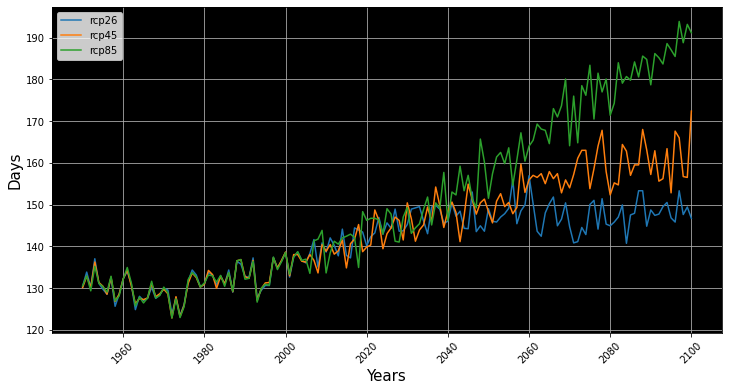
\includegraphics[scale=0.4]{ABfrost}
\caption{Consecutive Frost Free Days in Alberta}
\label{ABfrostdays}
\end{figure}

\begin{figure}[h!]
\centering
 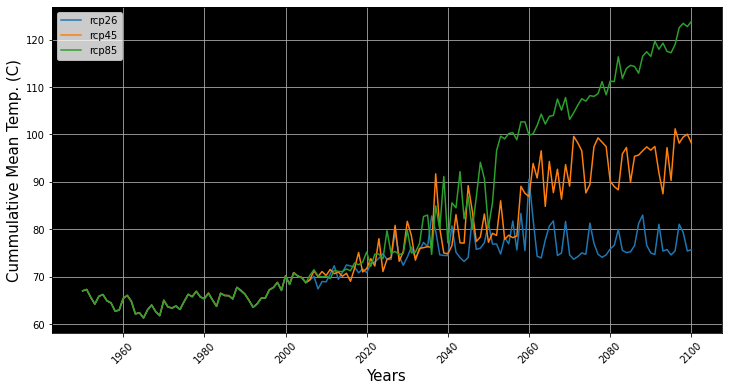
\includegraphics[scale=0.4]{ABtemp}
 \caption{cummulative Mean Temperatures in Alberta}
 \label{ABmeantemp}
\end{figure}

\begin{figure}[h!]
\centering
 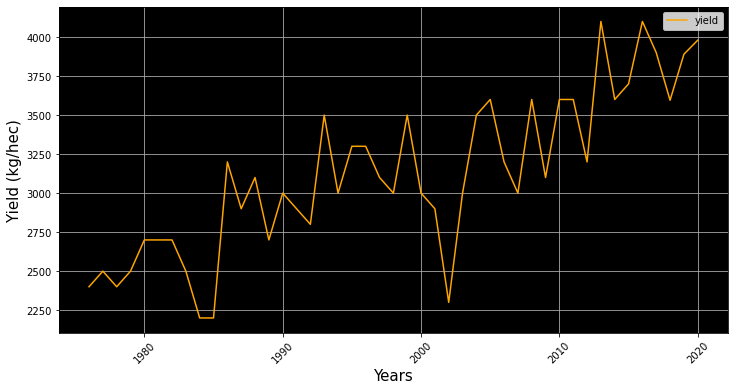
\includegraphics[scale=0.4]{AByield}
 \caption{Barley Yields in Alberta}
 \label{ABbarleyyields}
\end{figure}

\begin{figure}[h!]
 \centering
 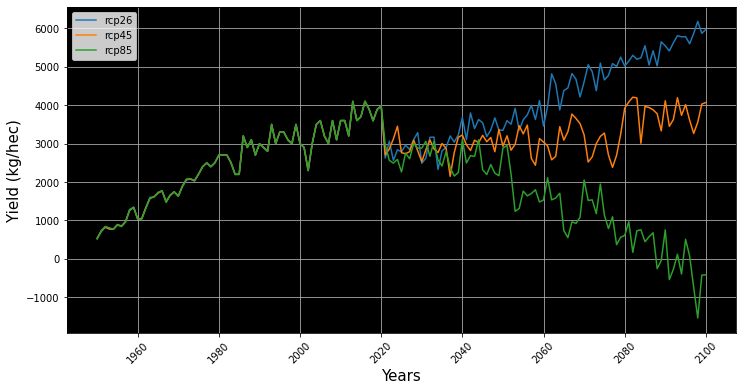
\includegraphics[scale=0.4]{ABproj}
 \caption{Projected Barley Yields in Alberta}
 \label{ABprojections}
\end{figure}

% ===============================================================================================
\begin{figure}[t]
\centering
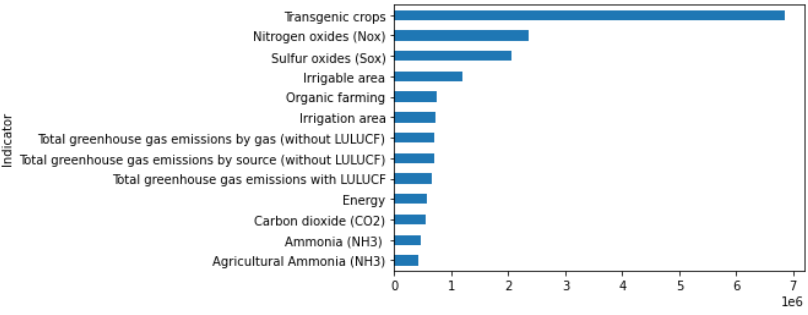
\includegraphics[width=0.50\paperwidth, clip=true, trim=0mm 0mm 0mm 0mm]{figures/Indicator_Value}\\

\caption{ Comparison of the different types of indicators  values in Canada, from 1984 to 2017. Shows only the indicators over the mean value, where transgenic crops was the most used indicator.
}
\label{Example1fig}
\end{figure}
% ===============================================================================================
% ===============================================================================================
\begin{figure}[t]
\centering
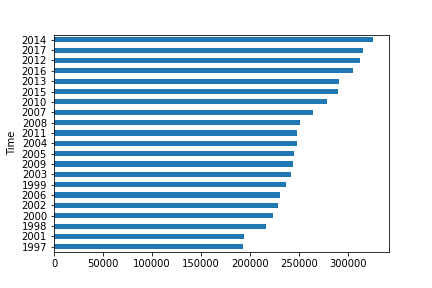
\includegraphics[width=0.30\paperwidth, clip=true, trim=0mm 0mm 0mm 0mm]{figures/Time_Value}\qquad

\caption{Shows  the amount of indicators per year from 1984 to 2017. The year were more  indicators were used was 2014 and 2017.
}
\label{Example2fig}
\end{figure}
% ===============================================================================================
% ===============================================================================================
\begin{figure}[t]
\centering
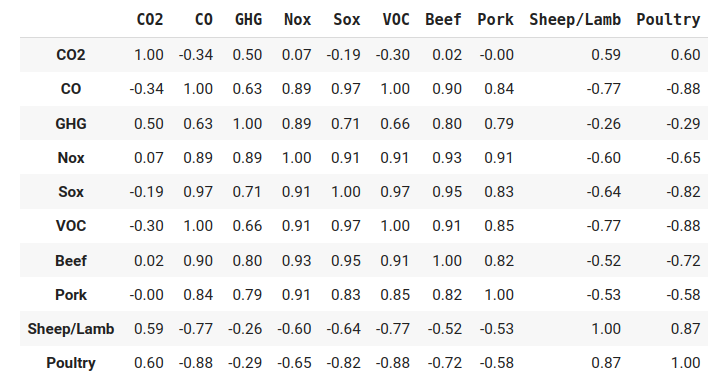
\includegraphics[width=0.30\paperwidth, clip=true, trim=0mm 0mm 0mm 0mm]{figures/corr}
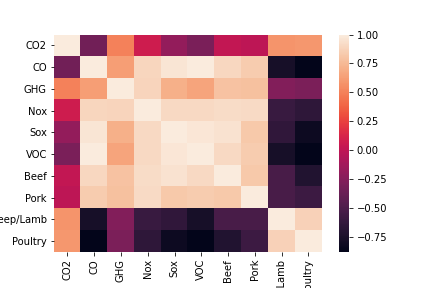
\includegraphics[width=0.30\paperwidth, clip=true, trim=0mm 0mm 0mm 0mm]{figures/matrix_1}

\caption{We compare different factors from environment impact with a correlation matrix. (\textbf{Left}) Shows the pairwise correlation  coefficients between various variables of the Canadian food production, such as GHG and farm supplies. (\textbf{Right}) Shows a visualization of the corresponding correlation matrix on the left.
}
\label{Example3fig}
\end{figure}
% ===============================================================================================
% ===============================================================================================
\begin{figure}[t]
\centering
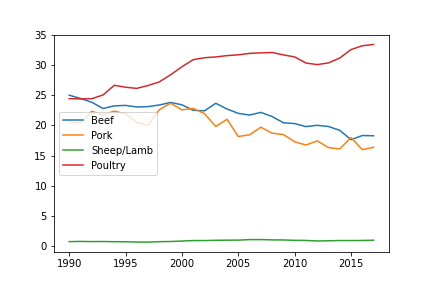
\includegraphics[width=0.30\paperwidth, clip=true, trim=0mm 0mm 0mm 0mm]{figures/graph_meat}
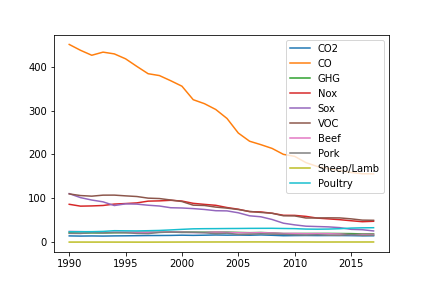
\includegraphics[width=0.30\paperwidth, clip=true, trim=0mm 0mm 0mm 0mm]{figures/graph_NEW}

\caption{Comparison in  time of food supplies production per-capita from 1990 to 2017. (\textbf{Left}) Shows the evolution of different products from farms, whereas we observe an increasing number of poultry but a decreasing number of other supplies as beef and pork. (\textbf{Right}) Shows the evolution of the farm products along GHG produced in the same time frame.
}
\label{Example4fig}
\end{figure}
% ===============================================================================================
% ===============================================================================================
\begin{figure}[t]
\centering
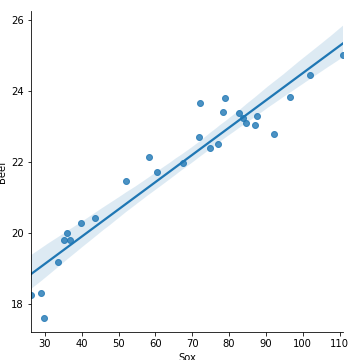
\includegraphics[width=0.30\paperwidth, clip=true, trim=0mm 0mm 0mm 0mm]{figures/Sox_Beef}
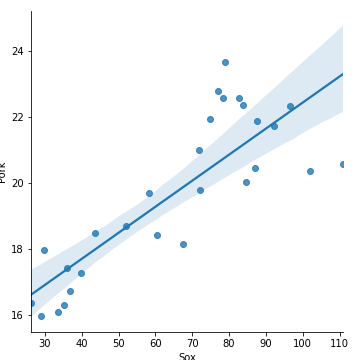
\includegraphics[width=0.30\paperwidth, clip=true, trim=0mm 0mm 0mm 0mm]{figures/Sox_Pork}

\caption{Shows  a best-fit line for two variables and the respective confidence intervals. (\textbf{Left}) Comparison for a linear correlation between beef production per-capita and Sox gas emited. (\textbf{Right}) Comparison for a linear correlation between pork production per-capita and Sox gas emited. 
}
\label{Example5fig}
\end{figure}
% ===============================================================================================
% ===============================================================================================
\begin{figure}[t]
\centering
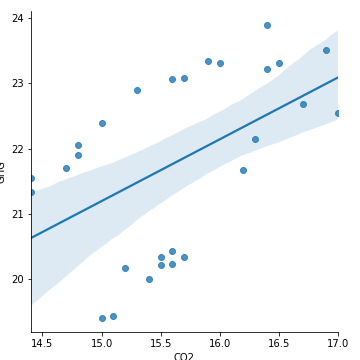
\includegraphics[width=0.30\paperwidth, clip=true, trim=0mm 0mm 0mm 0mm]{figures/corr_CO2_GHG}
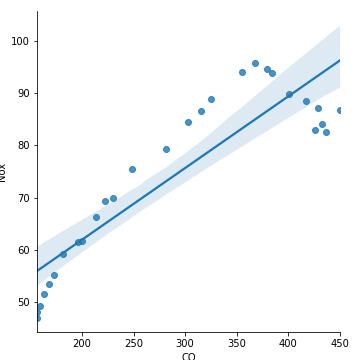
\includegraphics[width=0.30\paperwidth, clip=true, trim=0mm 0mm 0mm 0mm]{figures/corr_CO_NOX}

\caption{Shows  a best-fit line for GHG and one specific gas with the respective confidence intervals. (\textbf{Left}) Comparison for a linear correlation between GHG production per-capita and CO2  emited. (\textbf{Right}) Comparison for a linear correlation between GHG production per-capita and CO emited. 
}
\label{Example6fig}
\end{figure}
% ===============================================================================================

\end{document}

